\documentclass{article}
\usepackage[T1]{fontenc}
\usepackage{lmodern}
\usepackage{graphicx}
\usepackage{amsmath,amssymb}
\usepackage[a4paper,margin=2cm]{geometry}
\usepackage[absolute,overlay]{textpos}
\setlength{\TPHorizModule}{1mm}
\setlength{\TPVertModule}{1mm}
\usepackage[indonesian]{babel}
\usepackage{hyperref}
\setlength{\emergencystretch}{2em}
% unit: Halaman 40

\begin{document}

% === Halaman 40 (llm) ===

\section*{Elliptic Curve Diffie-Hellman (ECDH)}

\vspace{172.26mm}

Ingatlah kembali diagram pertukaran kunci Diffie-Hellman:

\vspace{60mm}

% deskripsi: Diagram pertukaran kunci Diffie-Hellman yang menunjukkan langkah-langkah komputasi antara Alice dan Bob, termasuk pembangkitan angka rahasia a dan b, perhitungan nilai publik A dan B, serta penghitungan kunci bersama K.
% bbox normalisasi: [0.2200, 0.3400, 0.6700, 0.9200]
\begin{textblock*}{94.50mm}(46.20mm,100.98mm)
\noindent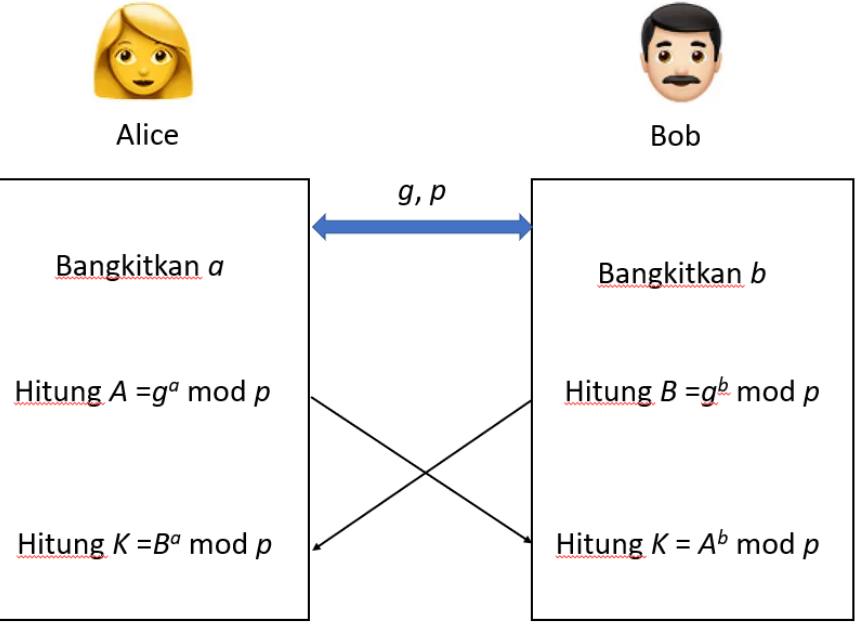
\includegraphics[width=94.50mm,height=172.26mm]{../../images/llm/page_040_img_01.png}%
\end{textblock*}

\end{document}
